\section*{Exercises}
\begin{enumerate}[\bfseries 1.]
\item Show that the following limit does not exitst \[
\lim_{z\to0}\Big(\frac{\bar z}{z}\Big)^2
\] Do this by letting nonzero points $z=(x,0)$ and $z=(x,x)$ approach the origin. (Note that it is not sufficient to simply consider points $z=(x,0)$ and $z=(0,y)$.)
\begin{proof}[\Sol]
Let $z=x+iy\in\C$ with $x,y\in\mathbb{R}$. Then \[
\left(\frac{\overline{z}}{z}\right)^{\!2}
=\left(\frac{x-iy}{x+iy}\right)^{\!2}.
\] If $z=re^{i\theta}$ with $r>0$, then $\bar z/z=e^{-2i\theta}$, so $|(\bar z/z)^2|=|e^{-4i\theta}|=1$.
\begin{center}
\begin{tikzpicture}[>=Latex,scale=1]
% =============== z-plane (paths to the origin) ===============
\begin{scope}
	% axes
	\draw[->] (-2.0,0) -- (2.0,0) node[right] {$\Re z$};
	\draw[->] (0,-2.0) -- (0,2.0) node[above] {$\Im z$};
	\node at (0,-2.25) {$z$-plane (approach $z\to 0$)};
	
	% origin as a hole (z=0 excluded)
	\fill[white] (0,0) circle (2.6pt);
	\draw[red] (0,0) circle (2pt) node[above right] {$z=0$ (undefined)};
	
	% Path 1: real axis y=0 (blue)
	\draw[blue!70,very thick,->] (-2,0) -- (-0.05,0) node[midway, above] {Path1: $y=0$};
	
	% Path 2: diagonal y=x (teal)
	\draw[teal!70,very thick,->] (-1.75,-1.75) -- (-0.05,-0.05) node[midway, xshift=-1.25cm] {Path2: $y=x$};
\end{scope}
% =============== mapping arrow ===============
\draw[->,thick] (3.5,0) -- (6,0)
node[midway,above] {$f(z)=\left(\dfrac{\overline z}{z}\right)^2$};
% =============== value plane (outputs) ===============
\begin{scope}[xshift=8.4cm]
	% axes
	\draw[->] (-2,0) -- (2,0) node[below right] {$\Re$};
	\draw[->] (0,-1.8) -- (0,1.8) node[left] {$\Im$};
	\node at (0,-2.05) {value plane of $f(z)$};
	
	% unit circle (context): |(\bar z/z)^2| = 1 for z≠0
	\draw[gray!40] (0,0) circle (1);
	
	% images of the two paths (constants 1 and -1)
	% Path 1 (y=0) -> 1
	\fill[blue!70] (1,0) circle (2.4pt) node[above right] {$1$};
	\draw[blue!70,->] (1.1,.75) to[bend left=10] (1,0);
	\node[blue!70,align=center] at (1,1.2)
	{along $y=0$:\\ $f(z)\equiv 1$};
	
	% Path 2 (y=x) -> -1
	\fill[teal!70] (-1,0) circle (2.4pt) node[below left] {$-1$};
	\draw[teal!70,->] (-1.1,-0.75) to[bend left=10] (-1,0);
	\node[teal!70,align=center] at (-1,-1.2)
	{along $y=x$:\\ $f(z)\equiv -1$};
	
%	% conclusion box
%	\node[draw,rounded corners=2pt,align=left,anchor=north] at (0,-1.25)
%	{$\displaystyle \lim_{z\to 0}\left(\frac{\overline z}{z}\right)^2\ \text{does not exist},$\\
%		since the limits along $y=0$ and $y=x$ differ.};
\end{scope}
\end{tikzpicture}
\end{center}
\medskip
\noindent\textbf{(1) Path 1: approach along the real axis $y=0$}

Let $z=x+0i=x$ with $x\in\mathbb{R}\setminus\{0\}$ and $x\to 0$. Then $
\displaystyle\left(\frac{\overline{z}}{z}\right)^2
=\left(\frac{x}{x}\right)^2
=1$.

\medskip
\noindent\textbf{(2) Path 2: approach along the diagonal $y=x$}

Let $z=x+ix=(1+i)x$ with $x\in\mathbb{R}\setminus\{0\}$ and $x\to 0$. Then
\[
\frac{\overline{z}}{z}
=\frac{\overline{(1+i)x}}{(1+i)x}
=\frac{(1-i)\,x}{(1+i)\,x}
=\frac{1-i}{1+i}
=\frac{(1-i)^2}{(1+i)(1-i)}
=\frac{1-2i+i^2}{1- i^2}
=\frac{1-2i-1}{2}
=\frac{-2i}{2}
=-i.
\]
Hence
\[
\left(\frac{\overline{z}}{z}\right)^2
=(-i)^2
=-1.
\] 

\medskip
\noindent\textbf{(3) Conclusion}

Since the limits along these two paths are different (namely $1$ and $-1$), the limit cannot exist.
\end{proof}
%	\item[X] Compute $\displaystyle \lim_{z\to\infty}\frac{4z^2}{(z-1)^2}$, $\ \lim_{z\to1}\frac{1}{(z-1)^3}$, and $\ \lim_{z\to\infty}\frac{z^2+1}{z-1}$.
%	\item[X] Suppose $f(z_0)=g(z_0)=0$ with $g'(z_0)\neq0$ and both derivatives exist. Prove
%	\[
%	\lim_{z\to z_0}\frac{f(z)}{g(z)}=\frac{f'(z_0)}{g'(z_0)}.
%	\]
\item Let \[
f(z)=\begin{cases} \bar z^2/z,& z\neq0,\\ 0,& z=0.\end{cases}
\] Show that if $z=0$, then $\Delta w/\Delta z=1$ at eatch nonzero point on the real and imaginary axes in the $\Delta z$, or $\Delta x\Delta y$, plane. Then show that $\Delta w/\Delta z=-1$ at each nonzero point $(\Delta x, \Delta y)$ on the line $\Delta y=\Delta x$ in that plane. Conclude from these observations that $f'(0)$ does not exist. Note that to obtain this result, it is not sufficient to consider only horizontal and vertical approaches to the origin in the $\Delta z$ plane.
\begin{proof}
Let $\frac{\Delta w}{\Delta z}
=\frac{f(\Delta z)-f(0)}{\Delta z}
\quad(\Delta z\neq 0)$. Since $f(0)=0$, for $\Delta z\neq0$, $\displaystyle
\frac{\Delta w}{\Delta z}
=\frac{f(\Delta z)}{\Delta z}
=\frac{\overline{\Delta z}^{\,2}}{(\Delta z)^2}$.

\medskip
\noindent\textbf{(1) Real and imaginary axes.}
\begin{itemize}
	\item Real axis: $\Delta z=x$ with $x\in\mathbb{R}\setminus\{0\}$, $\displaystyle
	\frac{\Delta w}{\Delta z}=\frac{\overline{x}^{\,2}}{x^2}=\frac{x^2}{x^2}=1$.
	\begin{center}
	\begin{tikzpicture}[>=Latex,scale=1.05]	
		%================ z-plane: explicit paths =================
		\begin{scope}
			% axes
			\draw[->] (-2,0) -- (2,0) node[right] {$\Re z$};
			\draw[->] (0,-2) -- (0,2) node[above] {$\Im z$};
			% hole at the origin (Delta z = 0 excluded)
			\fill[white] (0,0) circle (2.6pt);
			\draw[red] (0,0) circle (2pt) node[above right] {$\Delta z=0$ (excluded)};
			% Path A: real axis, Δz = x, x→0, x≠0
			\draw[line width=1.6pt,blue!70,->] (-2.8,0) -- (-0.12,0);
			\draw[line width=1.6pt,blue!70,->] ( 2.8,0) -- ( 0.12,0);
			\node[blue!70,anchor=north] at (0,-0.10)
			{$\displaystyle \text{Path A: }\Delta z=x,\ x\in\mathbb R\!\setminus\!\{0\},\ x\to 0$};
		\end{scope}
		%================ mapping arrow =================
		\draw[->,thick] (3.5,0) -- (7,0)
		node[midway,above] {$\displaystyle \frac{\Delta w}{\Delta z}=\frac{\overline{\Delta z}^{\,2}}{(\Delta z)^2}$};
		%================ value plane: constant images =================
		\begin{scope}[xshift=9.4cm]
			% axes
			\draw[->] (-2,0) -- (2,0) node[right] {$\Re f(z)$};
			\draw[->] (0,-2) -- (0,2) node[above] {$\Im f(z)$};
			%	\node at (0,-2.55) {$f(z)$-plane of $\Delta w/\Delta z$};
			% unit circle for context (|Δw/Δz|=1 for Δz≠0)
			\draw[gray!35] (0,0) circle (1);
			% Image of Path A (real axis): constant 1
			\fill[blue!70] (1,0) circle (2.6pt) node[above right] {$\displaystyle \text{Path A: } \frac{\overline{x}^{\,2}}{x^2}=1$};
		\end{scope}
	\end{tikzpicture}
	\end{center}
	\item Imaginary axis: $\Delta z=iy$ with $y\in\mathbb{R}\setminus\{0\}$, $\displaystyle
	\frac{\Delta w}{\Delta z}
	=\frac{\overline{iy}^{\,2}}{(iy)^2}
	=\frac{(-iy)^2}{(iy)^2}
	=\frac{-y^2}{-y^2}=1$.
	\begin{center}
	\begin{tikzpicture}[>=Latex,scale=1.05]	
		%================ z-plane: explicit paths =================
		\begin{scope}
			% axes
			\draw[->] (-2,0) -- (2,0) node[right] {$\Re z$};
			\draw[->] (0,-2) -- (0,2) node[above] {$\Im z$};
			% hole at the origin (Delta z = 0 excluded)
			\fill[white] (0,0) circle (2.6pt);
			\draw[red] (0,0) circle (2pt) node[above right] {$\Delta z=0$ (excluded)};
			% Path B: imaginary axis, Δz = iy, y→0, y≠0
			\draw[line width=1.6pt,purple!70,->] (0,-2.0) -- (0,-0.12);
			\draw[line width=1.6pt,purple!70,->] (0, 2.0) -- (0, 0.12);
			\node[purple!70,anchor=north] at (0,-2)
			{$\displaystyle \text{Path B: }\Delta z=iy,\ y\in\mathbb R\!\setminus\!\{0\},\ y\to 0$};
		\end{scope}
		%================ mapping arrow =================
		\draw[->,thick] (3.5,0) -- (7,0)
		node[midway,above] {$\displaystyle \frac{\Delta w}{\Delta z}=\frac{\overline{\Delta z}^{\,2}}{(\Delta z)^2}$};
		%================ value plane: constant images =================
		\begin{scope}[xshift=9.4cm]
			% axes
			\draw[->] (-2,0) -- (2,0) node[right] {$\Re f(z)$};
			\draw[->] (0,-2) -- (0,2) node[above] {$\Im f(z)$};
			%	\node at (0,-2.55) {$f(z)$-plane of $\Delta w/\Delta z$};
			% unit circle for context (|Δw/Δz|=1 for Δz≠0)
			\draw[gray!35] (0,0) circle (1);
			% Image of Path B (imag axis): constant 1
			\fill[purple!70] (1,0) circle (2.6pt);
			\node[purple!70,anchor=north west] at (0.95,-0.18)
			{$\displaystyle \text{Path B: } \frac{\overline{(iy)}^{\,2}}{(iy)^2}=1$};
		\end{scope}
	\end{tikzpicture}
	\end{center}
\end{itemize}

\noindent\textbf{(2) Line $\Delta y=\Delta x$.}
Let $\Delta z=(1+i)x$ with $x\in\mathbb{R}\setminus\{0\}$. Then
\[
\frac{\Delta w}{\Delta z}
=\frac{\overline{(1+i)x}^{\,2}}{((1+i)x)^2}
=\frac{((1-i)x)^2}{((1+i)x)^2}
=\frac{(1-i)^2}{(1+i)^2}
=\frac{-2i}{2i}=-1.
\]
\begin{center}
\begin{tikzpicture}[>=Latex,scale=1.05]	
%================ z-plane: explicit paths =================
\begin{scope}
	% axes
	\draw[->] (-2,0) -- (2,0) node[right] {$\Re z$};
	\draw[->] (0,-2) -- (0,2) node[above] {$\Im z$};
	%	\node at (0,-2.55) {$z$-plane (approach $\Delta z\to 0$)$\,$};	
	% hole at the origin (Delta z = 0 excluded)
	\fill[white] (0,0) circle (2.6pt);
	\draw[red] (0,0) circle (2pt) node[above right] {$\Delta z=0$ (excluded)};
	% Path C: diagonal Δy=Δx, i.e., Δz = (1+i)t, t→0, t≠0
	\draw[line width=1.6pt,teal!75,->] (-2.2,-2.2) -- (-0.12,-0.12);
	\draw[line width=1.6pt,teal!75,->] ( 2.2, 2.2) -- ( 0.12, 0.12);
	\node[teal!75,anchor=south east] at (5,-2.35)
	{$\displaystyle \text{Path C: }\Delta z=(1+i)t,\ t\in\mathbb R\!\setminus\!\{0\},\ t\to 0$};
\end{scope}
%================ mapping arrow =================
\draw[->,thick] (3.5,0) -- (7,0)
node[midway,above] {$\displaystyle 
	\frac{\Delta w}{\Delta z}=\frac{\overline{\Delta z}^{\,2}}{(\Delta z)^2}
	%	\displaystyle \,f(z)=\begin{cases}
		%		\overline z^{\,2}/z &\text{if}\; z\neq 0\\
		%		0 &\text{if}\; z=0
		%	\end{cases}
	$};
%================ value plane: constant images =================
\begin{scope}[xshift=9.4cm]
	% axes
	\draw[->] (-2,0) -- (2,0) node[right] {$\Re f(z)$};
	\draw[->] (0,-2) -- (0,2) node[above] {$\Im f(z)$};
	%	\node at (0,-2.55) {$f(z)$-plane of $\Delta w/\Delta z$};
	% Image of Path C (diagonal): constant -1
	\fill[teal!75] (-1,0) circle (2.6pt) node[below] {$\displaystyle \text{Path C: } \frac{\overline{(1+i)t}^{\,2}}{((1+i)t)^2}=-1$};
\end{scope}
\end{tikzpicture}
\end{center}
\medskip
\noindent\textbf{(3) Conclusion.}
Since the difference quotient equals $1$ along the axes but $-1$ along the line $\Delta y=\Delta x$, the limit
\[
\lim_{\Delta z\to 0}\frac{f(\Delta z)-f(0)}{\Delta z}
\]
depends on the path and therefore does not exist. Consequently, $f'(0)$ does not exist.
\end{proof}	
\newpage
\item Let \[
f(z)=\bar z,\quad f(z)=2x+ixy^2,\quad f(z)=e^{\bar z}
\] Then show that $f'(z)$ does not exists at any point.
\begin{proof}[\Sol]
Let \(z=x+iy\) and \(f(z)=u+iv\) with $x,y,u,v\in\R$. The Cauchy--Riemann equations \[
u_x=v_y,\qquad u_y=-\,v_x
\]
are necessary and sufficient for complex differentiability.

\medskip
\noindent\textbf{(1) \(f_1(z)=\overline z=\overline{x+iy}=x-iy\).}

Here \(u(x,y)=x,\ v(x,y)=-y\). Thus \[
u_x=1,\quad u_y=0,\quad v_x=0,\quad v_y=-1.
\]
The CR require \(u_x=v_y\), i.e.\ \(1=-1\), which is impossible. Hence \(f_1'\) does not exist anywhere.

\medskip
\noindent\textbf{(2) \(f_2(z)=2x+i\,x y^{2}\).}

Here \(u(x,y)=2x,\ v(x,y)=x y^{2}\). Thus
\[
u_x=2,\quad u_y=0,\quad v_x=y^{2},\quad v_y=2xy.
\]
The CR demand \[
\begin{cases} u_x=v_y\\ u_y=-v_x \end{cases}\implies
\begin{cases} 2=2xy\\ 0=y^2 \end{cases}\implies
\begin{cases} xy=1\\ y=0 \end{cases}.
\] These cannot hold simultaneously for any \(x\). Hence CR fail at every point, so \(f_2'\) exists nowhere.

\medskip
\noindent\textbf{(3) \(f_3(z)=e^{\overline z}\).}

Let \(\overline z=x-iy\). Then $f_3(x,y)=e^{x-iy}=e^{x}(\cos y-i\sin y)$, so \[
u(x,y)=e^{x}\cos y,\qquad v(x,y)=-\,e^{x}\sin y.
\] Compute \[
u_x=e^{x}\cos y,\quad u_y=-e^{x}\sin y,\quad
v_x=-e^{x}\sin y,\quad v_y=-e^{x}\cos y.
\] The CR give \[
\begin{cases} u_x=v_y\\ u_y=-v_x \end{cases}\implies
\begin{cases} e^x\cos y=-e^x\cos y\\ -e^x\sin y=+e^x\sin y \end{cases}\implies
\begin{cases} \cos y = 0\\ \sin y=0 \end{cases}.
\] These cannot hold simultaneously for any \(y\). Hence CR fail everywhere and \(f_3'\) exists nowhere.
\end{proof}
\item Let $f(z)=u(x,y)+i v(x,y)$ be given by \[
f(z)=\begin{cases}
	\bar z^2/z &: z\neq 0 \\
	0 &: z=0.
\end{cases}
\] Verify that the Cauchy--Riemann equations $u_x=v_y$ and $u_y=-v_x$ are satisfied at the origin $z=(0,0)$.
\begin{proof}
Write $z=x+iy$ and define
\[
f(z)=
\begin{cases}
	\dfrac{\overline z^{\,2}}{z}, & (x,y)\neq(0,0),\\[4pt]
	0, & (x,y)=(0,0).
\end{cases}
\]
Let $f=u+iv$. We compute the first-order partials of $u,v$ at $(0,0)$ by restricting to the
coordinate axes.

\medskip
\noindent\textbf{Along the $x$-axis ($y=0$):} For $x\neq0$,
\[
f(x,0)=\frac{\overline{x}^{\,2}}{x}=x,
\]
hence $u(x,0)=x$ and $v(x,0)=0$. Therefore
\[
u_x(0,0)=\lim_{h\to0}\frac{u(h,0)-u(0,0)}{h}
=\lim_{h\to0}\frac{h-0}{h}=1,
\quad
v_x(0,0)=\lim_{h\to0}\frac{v(h,0)-v(0,0)}{h}
=\lim_{h\to0}\frac{0-0}{h}=0.
\]

\medskip
\noindent\textbf{Along the $y$-axis ($x=0$):} For $y\neq0$,
\[
f(0,y)=\frac{\overline{iy}^{\,2}}{iy}=\frac{(-iy)^2}{iy}=\frac{-y^2}{iy}=iy,
\]
so $u(0,y)=0$ and $v(0,y)=y$. Hence
\[
u_y(0,0)=\lim_{k\to0}\frac{u(0,k)-u(0,0)}{k}
=\lim_{k\to0}\frac{0-0}{k}=0,
\quad
v_y(0,0)=\lim_{k\to0}\frac{v(0,k)-v(0,0)}{k}
=\lim_{k\to0}\frac{k-0}{k}=1.
\]

\medskip
Thus at $(0,0)$ we have
\[
u_x(0,0)=1,\qquad v_y(0,0)=1,\qquad u_y(0,0)=0,\qquad v_x(0,0)=0,
\]
and consequently the Cauchy--Riemann equations
\(
u_x=v_y
\)
and
\(
u_y=-v_x
\)
hold at the origin.

\begin{remark}
	Although the Cauchy--Riemann equations hold at $(0,0)$, the complex derivative $f'(0)$ does not exist
	(since $\frac{f(\Delta z)-f(0)}{\Delta z}=\frac{\overline{\Delta z}^{\,2}}{(\Delta z)^2}$ takes different
	values along different approach directions).
\end{remark}
\end{proof}
\item Let \[
f(z)=\sin x\cosh y+i\cos x\sinh y\quad\text{and}\quad f(z)=e^{-y}(\sin x-i\cos x).
\] Then show that all $f$ are entire.
\begin{proof}[\sol]
Let \begin{align*}
f_1(z)&=\sin x\cosh y+i\cos x\sinh y\quad\text{and}\\
f_2(z)&=e^{-y}(\sin x-i\cos x).
\end{align*}
\textbf{(a) } 
Let $z = x + iy$ with $x,y \in \mathbb{R}$. Note that \[
\begin{array}{lcr}
	e^{iz}=\cos z+i\sin z && \displaystyle\cos z = \frac{e^{iz} + e^{-iz}}{2} \\
	&\longleftrightarrow& \\
	e^{-iz}=\cos z-i\sin z && \displaystyle\sin z = \frac{e^{iz} - e^{-iz}}{2i}
\end{array}
\]By definition,
\[
\sin z = \frac{e^{iz} - e^{-iz}}{2i}.
\]
Substitute $z = x + iy$:
\[
iz = i(x+iy) = ix - y, \qquad -iz = -ix + y,
\]
so
\[
e^{iz} = e^{ix-y} = e^{-y}e^{ix}, \qquad e^{-iz} = e^{-ix+y} = e^{y}e^{-ix}.
\]
Using Euler's formula $e^{ix} = \cos x + i\sin x$ and $e^{-ix} = \cos x - i\sin x$, we get
\[
e^{iz} = e^{-y}(\cos x + i\sin x), \qquad
e^{-iz} = e^{y}(\cos x - i\sin x).
\]
Then
\begin{align*}
	e^{iz} - e^{-iz}
	&= e^{-y}(\cos x + i\sin x) - e^{y}(\cos x - i\sin x) \\
	&= \cos x(e^{-y} - e^{y}) + i\sin x(e^{-y} + e^{y}).
\end{align*}
Recall the hyperbolic functions
\[
\cosh y = \frac{e^{y} + e^{-y}}{2}, \qquad
\sinh y = \frac{e^{y} - e^{-y}}{2},
\]
so that
\[
e^{-y} + e^{y} = 2\cosh y, \qquad
e^{-y} - e^{y} = -2\sinh y.
\]
Hence
\begin{align*}
	e^{iz} - e^{-iz}
	&= \cos x(-2\sinh y) + i\sin x(2\cosh y) \\
	&= 2\bigl(i\sin x\cosh y - \cos x\sinh y\bigr).
\end{align*}
Therefore
\begin{align*}
	\sin z
	&= \frac{e^{iz} - e^{-iz}}{2i}
	= \frac{2\bigl(i\sin x\cosh y - \cos x\sinh y\bigr)}{2i} \\
	&= \frac{i\sin x\cosh y}{i} - \frac{\cos x\sinh y}{i} \\
	&= \sin x\cosh y + i\cos x\sinh y,
\end{align*}
since $\dfrac{1}{i} = -i$.

Thus
\[
\boxed{\sin(x+iy) = \sin x \cosh y + i \cos x \sinh y.}
\]


Using the standard identity for the complex sine,
\[
\sin z=\sin(x+iy)=\sin x\cosh y + i\cos x\sinh y,
\]
we see immediately that $f_1(z)=\sin z$. Since $\sin z$ is an entire function (power series with infinite radius of convergence), $f_1$ is entire.

\smallskip
\textbf{(b) } Note that
\[
e^{iz}=e^{i(x+iy)}=e^{ix-y}=e^{-y}\bigl(\cos x + i\sin x\bigr).
\]
Multiplying by $-i$ gives
\[
-i\,e^{iz}=e^{-y}\bigl(\sin x - i\cos x\bigr)=f_2(z).
\]
Thus $f_2(z)=-i\,e^{iz}$. Since the exponential is entire and multiplication by a constant preserves holomorphy, $f_2$ is entire.

\smallskip
Therefore both functions are entire.
\end{proof}
	\newpage	
	\item Show that the function \[
	f(z)=\ln r+i\theta\quad (r>0,\; 0<\theta<2\pi)
	\] is analytic in the indicated domain of definition, with derivative $f'(z)=1/z$. Then show that th e composite function $g(z)=f(z^2+1)$ is analytic in the quadratic $x>0,y>0$ with derivative \[
	g'(z)=\frac{2z}{z^2+1}.
	\] (Suggestion: Observe that $\Im(z^2+1)>0$ when $x>0, y>0$)
\begin{proof}[\sol]
	Let $z=x+iy=re^{i\theta}$ with $r=\sqrt{x^2+y^2}>0$ and $0<\theta<2\pi$. Define
	\[
	f(z)=\ln r+i\theta .
	\]
	Then $f$ is analytic on the slit plane
	\begin{center}
	\begin{minipage}{.475\textwidth} \[
	\Omega:=\{\,z\in\mathbb{C}: r>0,\ 0<\theta<2\pi\,\}=\mathbb{C}\setminus[0,\infty),
	\] and $f'(z)=\frac{1}{z}\; (z\in\Omega)$.
	\end{minipage}\hfill
	\begin{minipage}{.475\textwidth}\centering
	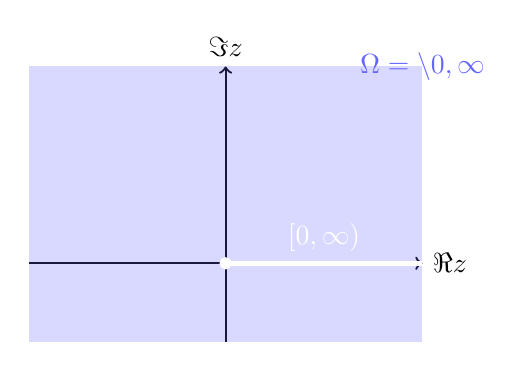
\begin{tikzpicture}
		% axes
		\draw[->, thick] (-2.5,0) -- (2.5,0) node[right] {$\Re z$};
		\draw[->, thick] (0,-1) -- (0,2.5) node[above] {$\Im z$};
		% shade domain
		\fill[blue!60, opacity=.25] (-2.5,-1) rectangle (2.5,2.5);
		\node[blue!60] at (2.5,2.5) {$\Omega=\C\setminus\intco{0,\infty}$};
		% slit: [0, +∞) on real axis
		\filldraw[white] (0,0) circle (2pt);
		\draw[white,ultra thick] (0,0) -- (2.5,0) node[midway, above] {$[0,\infty)$};
	\end{tikzpicture}
	\end{minipage}
	\end{center}
	Write $f=u+iv$ with \[
	u(x,y)=\ln r=\frac12\ln(x^2+y^2),\qquad v(x,y)=\theta=\Arg(z)\in(0,2\pi).
	\]
	On $\Omega$ the functions $u,v$ are $C^1$ and their partials are:
	\[
	u_x=\frac{x}{x^2+y^2},\quad u_y=\frac{y}{x^2+y^2},\qquad
	v_x=-\frac{y}{x^2+y^2},\quad v_y=\frac{x}{x^2+y^2}.
	\]
	Hence the Cauchy--Riemann equations hold on $\Omega$:
	\[
	u_x=v_y=\frac{x}{x^2+y^2},\qquad u_y=-v_x=\frac{y}{x^2+y^2}.
	\]
	Since these partials are continuous on $\Omega$, $f$ is analytic there. Its complex derivative is
	\[
	f'(z)=u_x+iv_x=\frac{x}{x^2+y^2}+i\!\left(-\frac{y}{x^2+y^2}\right)
	=\frac{x-iy}{x^2+y^2}=\frac{1}{x+iy}=\frac{1}{z}.
	\]
	For $g(z)=f(z^2+1)$, compute
	\begin{align*}
	z^2+1&=(x+iy)^2+1\\
	&=(x^2-y^2+2ixy) +1 \\
	&=(x^2-y^2+1)+i(2xy).
	\end{align*}
	If $x>0$ and $y>0$, then $\Im(z^2+1)=2xy>0$, so $z^2+1$ lies in the open upper half-plane $\mathbb{H}$, in particular in $\Omega$ (its argument lies in $(0,\pi)\subset(0,2\pi)$). 
	\begin{center}
	\begin{tikzpicture}[>=Latex,scale=.75]
		% ================= z-plane: domain Q =================
		\begin{scope}
			% axes
			\draw[->] (-0.6,0) -- (3.2,0) node[right] {$\Re z=x$};
			\draw[->] (0,-0.6) -- (0,3.0) node[above] {$\Im z=y$};
			\node at (1.6,-1.25) {$z$-plane};
			
			% shade first quadrant Q: x>0, y>0
			\fill[blue!12, opacity=.25] (0,0) rectangle (3.0,2.8);
			\node[blue!70] at (2.6,2.5) {$Q_1$};
			
			% sample point z = 1 + 0.8 i
			\fill[blue!80] (1.0,0.8) circle (2pt) node[above right] {$z$};
		\end{scope}
		% arrow z -> w
		\draw[->,thick] (5.6,1.4) -- (9.2,1.4) node[midway,above] {$w=z^2+1$};
		% ================= w-plane: image in upper half-plane, slit shown =================
		\begin{scope}[xshift=12.6cm]
			% axes
			\draw[->] (-2.6,0) -- (3.4,0) node[right] {$\Re w$};
			\draw[->] (0,-0.6) -- (0,3.0) node[above] {$\Im w$};
			\node at (0,-1.25) {$w$-plane};
			
			% shade upper half-plane Im w>0
			\fill[green!12, opacity=.25] (-2.5,0) rectangle (3.2,2.8);
			\node[green!60] at (2.5,2.5) {$\Im w>0$};
			
			% slit: [0, +∞) on real axis
			\draw[red!70,very thick] (0,0) -- (3.2,0) node[midway, below] {$[0,\infty)$};
%			\node[gray!70,anchor=west] at (-2.5,-0.35) {$\Omega=\C\setminus[0,\infty)$};
			% image of the sample point: z=1+0.8i -> w=(1-0.64+1)+i(2*1*0.8) = 1.36 + 1.6 i
			\fill[green!80!black] (1.36,1.60) circle (2.2pt) node[above right] {$w=z^2+1$};
			% guide from origin showing |w| and Arg(w)
			\draw[gray!60,dashed] (0,0) -- (1.36,1.60);
%			\node[gray!70] at (0.75,0.18) {$\Arg w\in(0,\pi)$};
		\end{scope}
		% arrow w -> s
		\draw[->,thick] (5.6,1.4-7) -- (9.2,1.4-7) node[midway,above] {$s=f(w)=\Log w$};
		% ================= s-plane: image strip 0<Im s<pi =================
		\begin{scope}[xshift=12.6cm, yshift=-7cm]
			% axes
			\draw[->] (-2.4,0) -- (3.2,0) node[right] {$\Re s=u$};
			\draw[->] (0,-0.6) -- (0,3.6) node[above] {$\Im s=v$};
			\node at (0,-1.25) {$s$-plane};
			% horizontal strip 0 < v < pi
			\fill[yellow!18, opacity=.25] (-2.3,0.00) rectangle (3.0,3.1416);
			\draw[gray!70] (-2.3,0.00) -- (3.0,0.00) node[right] {$v=0$};
			\draw[gray!70] (-2.3,3.1416) -- (3.0,3.1416) node[right] {$v=\pi$};
			\node[brown!70] at (2.4,2.8) {$0<\Im s<\pi$};
			% image of the sample w under Log: s = ln|w| + i Arg(w)
			% |w| ≈ sqrt(1.36^2+1.6^2) ≈ 2.100 -> ln|w| ≈ 0.741, Arg ≈ atan(1.6/1.36) ≈ 0.864
			\fill[brown!80!black] (0.741,0.864) circle (2.2pt)
			node[above right] {$s=\Log w$};
		\end{scope}
%		
%		% ================= footer: analyticity & derivative =================
%		\node[align=left] at (8.6,-0.9)
%		{\small In $Q$: $w=z^2+1$ has $\Im w=2xy>0\Rightarrow w\in\Omega$;\ \ $f=\Log$ is analytic on $\Omega$.\\
%			\small Hence $g(z)=f(z^2+1)$ is analytic on $Q$, and by chain rule
%			$\displaystyle\ g'(z)=f'(z^2+1)\cdot(2z)=\frac{2z}{z^2+1}\,.$};
%		
	\end{tikzpicture}
	\end{center}
	Thus $g$ is the composition of analytic functions on the first quadrant $Q_1$, hence analytic on $Q_1$. By the chain rule, \[
	g'(z)=f'(z^2+1)\cdot(2z)=\frac{2z}{z^2+1}\qquad (z\in Q_1).
	\]
\end{proof}
%	\item Find harmonic conjugates for $u(x,y)=2x-x^3+3xy^2$ and for $u(x,y)=\sinh x\sin y$.
%	\item If $v$ is a harmonic conjugate of $u$ and $u$ a harmonic conjugate of $v$ in $D$, show $u,v$ are constant in $D$.
%	\item Using polar CR, prove that for analytic $f=u+iv$ on $D\subset\C\setminus\{0\}$, $u$ satisfies $r^2u_{rr}+ru_r+u_{\theta\theta}=0$ (polar Laplace equation). Same for $v$.
%	\item Verify $u(r,\theta)=\ln r$ is harmonic on $r>0$, $0<\theta<2\pi$ and $v(r,\theta)=\theta$ is a harmonic conjugate.
%	\item If $f=u+iv$ is analytic on $D$, prove the level curves $u=c_1$ and $v=c_2$ intersect orthogonally at any point where $f'\neq0$.
\end{enumerate}
\newpage